

We illustrate the linguistic predictions of our theoretical results on the Memory-Surprisal tradeoff by reanalyzing the data from \cite{fedzechkina-human-2017}.
This is a miniature artificial language study that showed a bias for Dependency Length Minimization in production in artificial language learning.
Due to the controlled setting, it is possible to exactly compute the speaker's memory as given in Theorem~\ref{prop:suboptimal}.


As the bound in Theorem~\ref{prop:suboptimal} is invariant under reversal of the language, we only consider the head-final version of her artificial language.
The language has consistent head-final order, and uses case marking on objects.
The relevant production targets are transitive sentences where one of the two arguments is much longer than the other, due to the presence of a PP modifier, as shown in Table~\ref{tab:artificial}.
The language has variable order of subjects and objects; for the production targets, the B versions produce much longer dependencies than the A versions.
Dependency Length Minimization thus predicts that speakers are more likely to use the A versions.
\cite{fedzechkina-human-2017} confirmed this experimentally.


\begin{table}
	\textbf{A Orders: Short Dependencies}

		\begin{tabular}{ccc}
			Object & Subject & Verb \\
			\fbox{\begin{tabular}{llllll}
				\fbox{\begin{tabular}{llll} Adjective &Noun &Postposition\end{tabular}} & Noun-Case
					\end{tabular}} & \fbox{\begin{tabular}{l}Noun\end{tabular}} & \fbox{\begin{tabular}{l}Verb\end{tabular}}  \\
		\end{tabular}
\\
		\begin{tabular}{ccc}
			Subject & Object & Verb \\
			\fbox{\begin{tabular}{llllll}
				\fbox{\begin{tabular}{llll} Adjective &Noun &Postposition\end{tabular}} & Noun
					\end{tabular}} & \fbox{\begin{tabular}{l}Noun-Case\end{tabular}} & Verb \\
		\end{tabular}
\\
\\

	\textbf{B Orders: Long Dependencies}


		\begin{tabular}{ccc}
			Subject & Object & Verb \\
			 \fbox{\begin{tabular}{l}Noun\end{tabular}} &  \fbox{\begin{tabular}{llllll}
				\fbox{\begin{tabular}{llll} Adjective &Noun &Postposition\end{tabular}} & Noun-Case
		\end{tabular}}  &  \fbox{\begin{tabular}{l}Verb\end{tabular}}  \\
		\end{tabular}
\\
		\begin{tabular}{ccc}
			Object & Subject & Verb \\
			\fbox{\begin{tabular}{l}Noun-Case\end{tabular}} & \fbox{\begin{tabular}{llllll}
				\fbox{\begin{tabular}{llll} Adjective &Noun &Postposition\end{tabular}} & Noun
		\end{tabular}} & Verb \\
		\end{tabular}

			\caption{Production targets in the artificial mini language from \cite{fedzechkina-human-2017}. The language has head-final order, with free variation between SO and OS orders. When one of the arguments is much longer than the other, placing the longer one first (`A' orders) shortens syntactic dependencies, compared to `B' orders.}\label{tab:artificial}

\end{table}

In this section, we show that our bound on speaker memory makes the same prediction, without reference to syntactic structure or specific memory architectures. 

We constructed one language consisting of the A versions, and one language consisting of the B versions.
Following the experimental setup of \cite{fedzechkina-human-2017}, we assigned equal probability to the two possible configurations per language, and used a separate set of nouns (inanimate nouns) for the embedded noun in the long phrase.

We interpreted each of the two languages as a stationary processes, extending infinitely in both directions, by concatenating independent samples drawn from the language.
			We computed (\ref{eq:memory-bound}) from a chain of 1000 independently sampled sentences, for each of the two versions of the toy language.
			Figure~\ref{fig:toy-mis} (left) shows the curve of the conditional mutual information $I_t$ as a function of the distance $t$.
			The curves differ at $t=2$ and $t=5$: 
			About 0.073 nats of predictive information that are at distance $t=2$ in the A orders are moved to $t=5$ in the B orders.
%			In this sense, A orders have greater information locality than the B orders.
			%What is responsible for this difference?
			The source of the difference lies in predicting the presence and absence of a case marker on the second argument -- i.e., whether to anticipate a subject or object.
			In the A orders, considering the last two words is sufficient to make this decision.
			In the B orders, it is necessary to consider the word before the long second constituent, which is five words in the past.

			The total amounts of predictive information -- corresponding to the area under the curve -- are the same, indicating that both languages are equally predictable.
			However, we will see that the memory demands are different:
			Figure~\ref{fig:toy-mis} (right) shows $t\cdot I_t$ as a function of $t$.
			As $I_t$ decays faster in A orders, the total area under the curve now differs between A and B, and is larger in B.
			%This area corresponds to the lower bound in (\ref{eq:memory-bound}), and is 2.21 nats in A orders, and 2.43 nats in B orders.

%While (\ref{eq:memory-bound}) is a general lower bound, it can be proven that this bound is actually tight in the case of this specific example.\footnote{This can be shown by computing the causal states and then showing that the crypticity is zero, both of which is tractable in the case of this small-scale artificial language.}
%That is, a speaker who optimally allocates memory resources will spend 2.21 nats in A orders, and 2.43 nats in B orders.


In Figure~\ref{fig:toy-listener-tradeoff}, we show the resulting curve for the two versions of the artificial language from \cite{fedzechkina-human-2017}.
%In this language, speaker memory coincides with the memory demand of a listener who performs optimally in incremental prediction.
The curve shows that, at any desired level of surprisal, Order A requires at most as much memory as Order B.
For reaching optimal surprisal, Order A requires strictly less memory.
Thus, in this case, the listener's surprisal-memory tradeoff is optimized by the orders predicted by Dependency Length Minimization.

It is important to stress that, even though we computed this value by considering the number of words impacting predictions at a given point in time, this bound holds independently of the actual implementation and architecture of memory and predictions.




\begin{figure*}
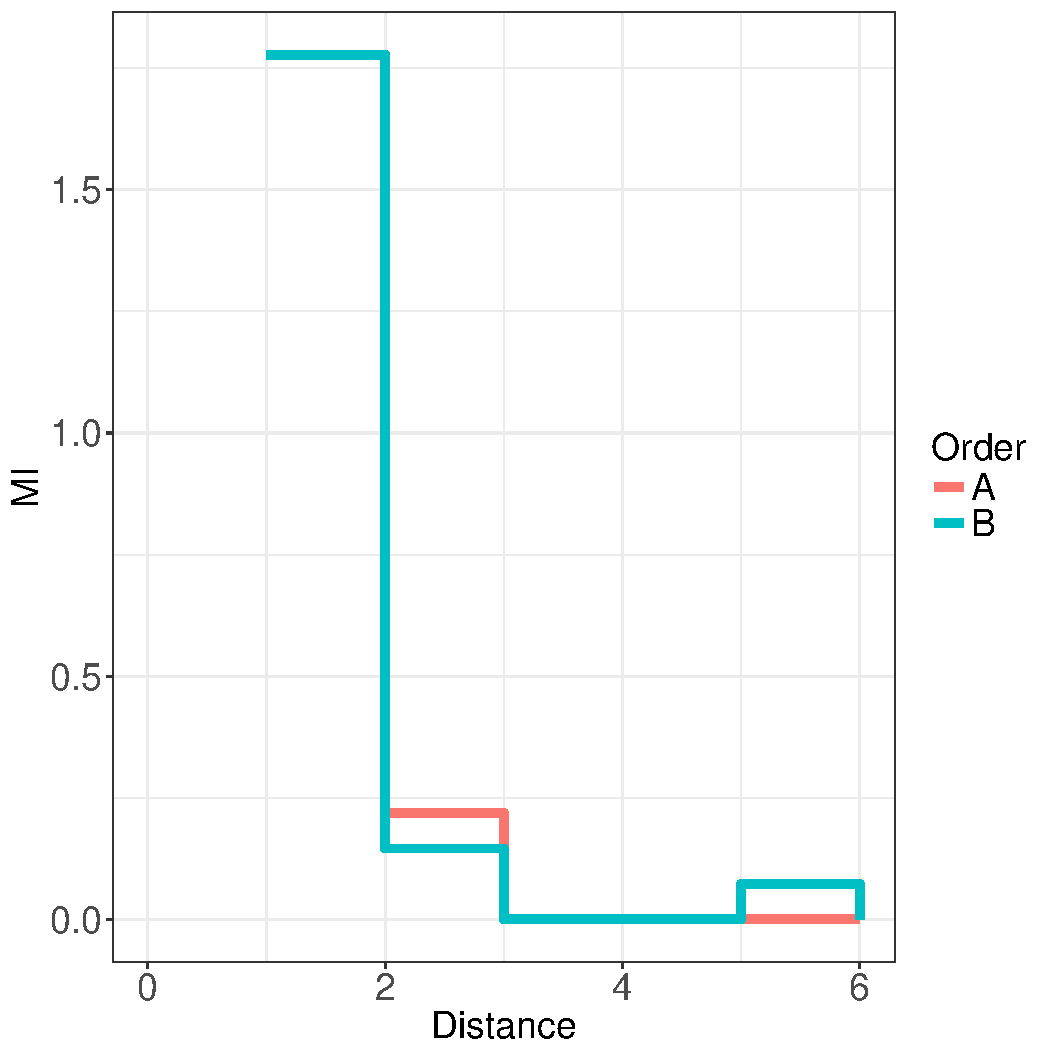
\includegraphics[width=0.45\textwidth]{../code/toy/figures/toy-mis.pdf}
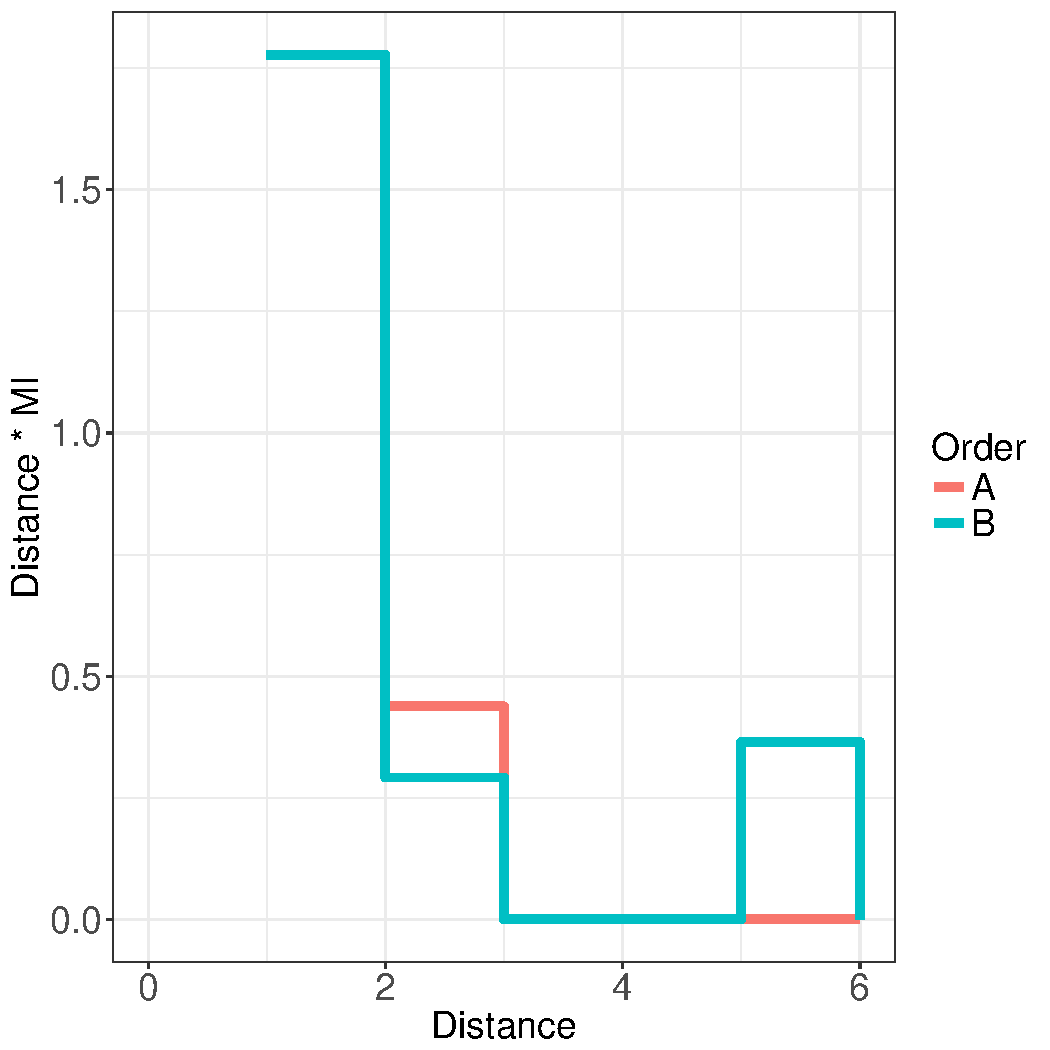
\includegraphics[width=0.45\textwidth]{../code/toy/figures/toy-t-mis.pdf}
%
	\caption{Left: Decay of Conditional Mutual Information, as a function of the distance $t$, for the two versions in the artificial language. The areas under the two curves are identical, corresponding to the fact that both orders are equally predictable. However, mutual Information decays faster in Order A.\ \ \ Right: $t I_t$, as a function of $t$. The area under the B curve is larger, corresponding to larger memory demand for this order.}\label{fig:toy-mis}
\end{figure*}
%Both languages have the same overall entropy rate, but they differ in the distribution of predictive information.
%
%plot of $I_t$
%
%The areas under the curves are identical.
%
%good version
%
%%CONTEXT LENGTH 0   2.06856758681  9997.93143241   0.0
%%CONTEXT LENGTH 1   0.29195106479  1.77661652202   1.77661652202
%%CONTEXT LENGTH 2   0.0729865489103  0.21896451588   2.21454555377
%%CONTEXT LENGTH 3   0.0729865489103  0.0   2.21454555377
%%CONTEXT LENGTH 4   0.0729865489103  0.0   2.21454555377
%%CONTEXT LENGTH 5   0.0729865489103  0.0   2.21454555377
%%CONTEXT LENGTH 6   0.0729865489103  0.0   2.21454555377
%
%bad version
%
%%CONTEXT LENGTH 0   2.06937301571  9997.93062698   0.0
%%CONTEXT LENGTH 1   0.291673373027  1.77769964269   1.77769964269
%%CONTEXT LENGTH 2   0.145830550934  0.145842822093   2.06938528687
%%CONTEXT LENGTH 3   0.145830550934  0.0   2.06938528687
%%CONTEXT LENGTH 4   0.145830550934  0.0   2.06938528687
%%CONTEXT LENGTH 5   0.0729152754672  0.0729152754672   2.43396166421
%%CONTEXT LENGTH 6   0.0729152754672  0.0   2.43396166421
%%CONTEXT LENGTH 7   0.0729152754672  0.0   2.43396166421
%%
%
%
%
%%
%%grammar:
%%
%%S $\rightarrow$ Obj Subj V (1/2) | Subj Obj V (1/2)
%%
%%Obj $\rightarrow$ NP di
%%
%%Subj $\rightarrow$ NP
%%
%%NP $\rightarrow$ N (3/4) | PP NP (1/8) | Adj NP (1/8)
%%
%%PP $\rightarrow$ NP P
%%
%
%

\begin{figure}
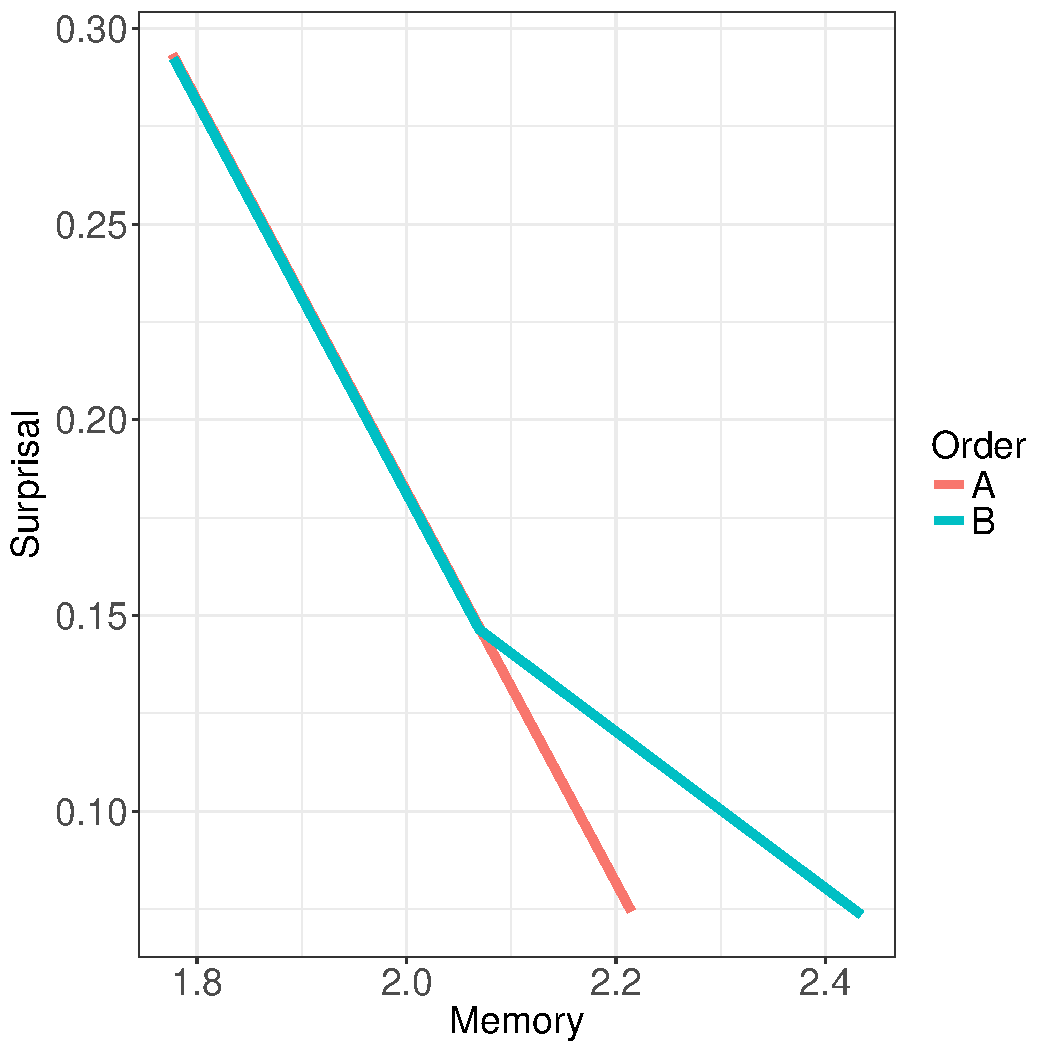
\includegraphics[width=0.45\textwidth]{../code/toy/figures/toy-mem-surp.pdf}
	\caption{Tradeoff between listener memory and surprisal, for the two versions of the artificial language from \cite{fedzechkina-human-2017}. Language A requires less memory at the same level of surprisal.}\label{fig:toy-listener-tradeoff}
\end{figure}


